




\section{Results}
\label{sec:centroidal_mpc_results}
In this section, we present the validation results of the control strategy presented in Section~\ref{sec:reduced_mpc}.
CasADi~\citep{Andersson2018CasADi:Control} and IPOPT 3.13.4~\citep{IPOpt2006} with HSL\_MA97~\citep{Hogg2011HSL_MA97Systems} libraries are used to solve the non-linear optimization problem. The code is written in pure C++ and is available at~\href{https://github.com/ami-iit/paper_romualdi_2022_icra_centroidal-mpc-walking}{\texttt{https://github.com/ami-iit/paper\_romualdi\_2022\_icra\_centroidal-mpc-walking}}.
\par
To validate the performance of the proposed control, we present two main experiments. First, we test the centroidal MPC considering only the centroidal Dynamics~\eqref{eq:centroidal_dynamics} for a one-leg and two-legs floating base systems. Secondly, we present the results obtained with the implementation of the control architecture shown in Figure~\ref{fig:centroidal_mpc_architecture} on the iCub Humanoid Robot V3 -- Section~\ref{sec:iCub3}. 
In both scenarios, we analyze the performance of the controller while running on a $10^\text{th}$ generation Intel$^\text{\textregistered}$ Core i7-10750H laptop equipped with Ubuntu Linux 20.04. 
\par
\begin{figure}[!t]
    \centering
    \begin{myframe}{One-leg jumping robot}
    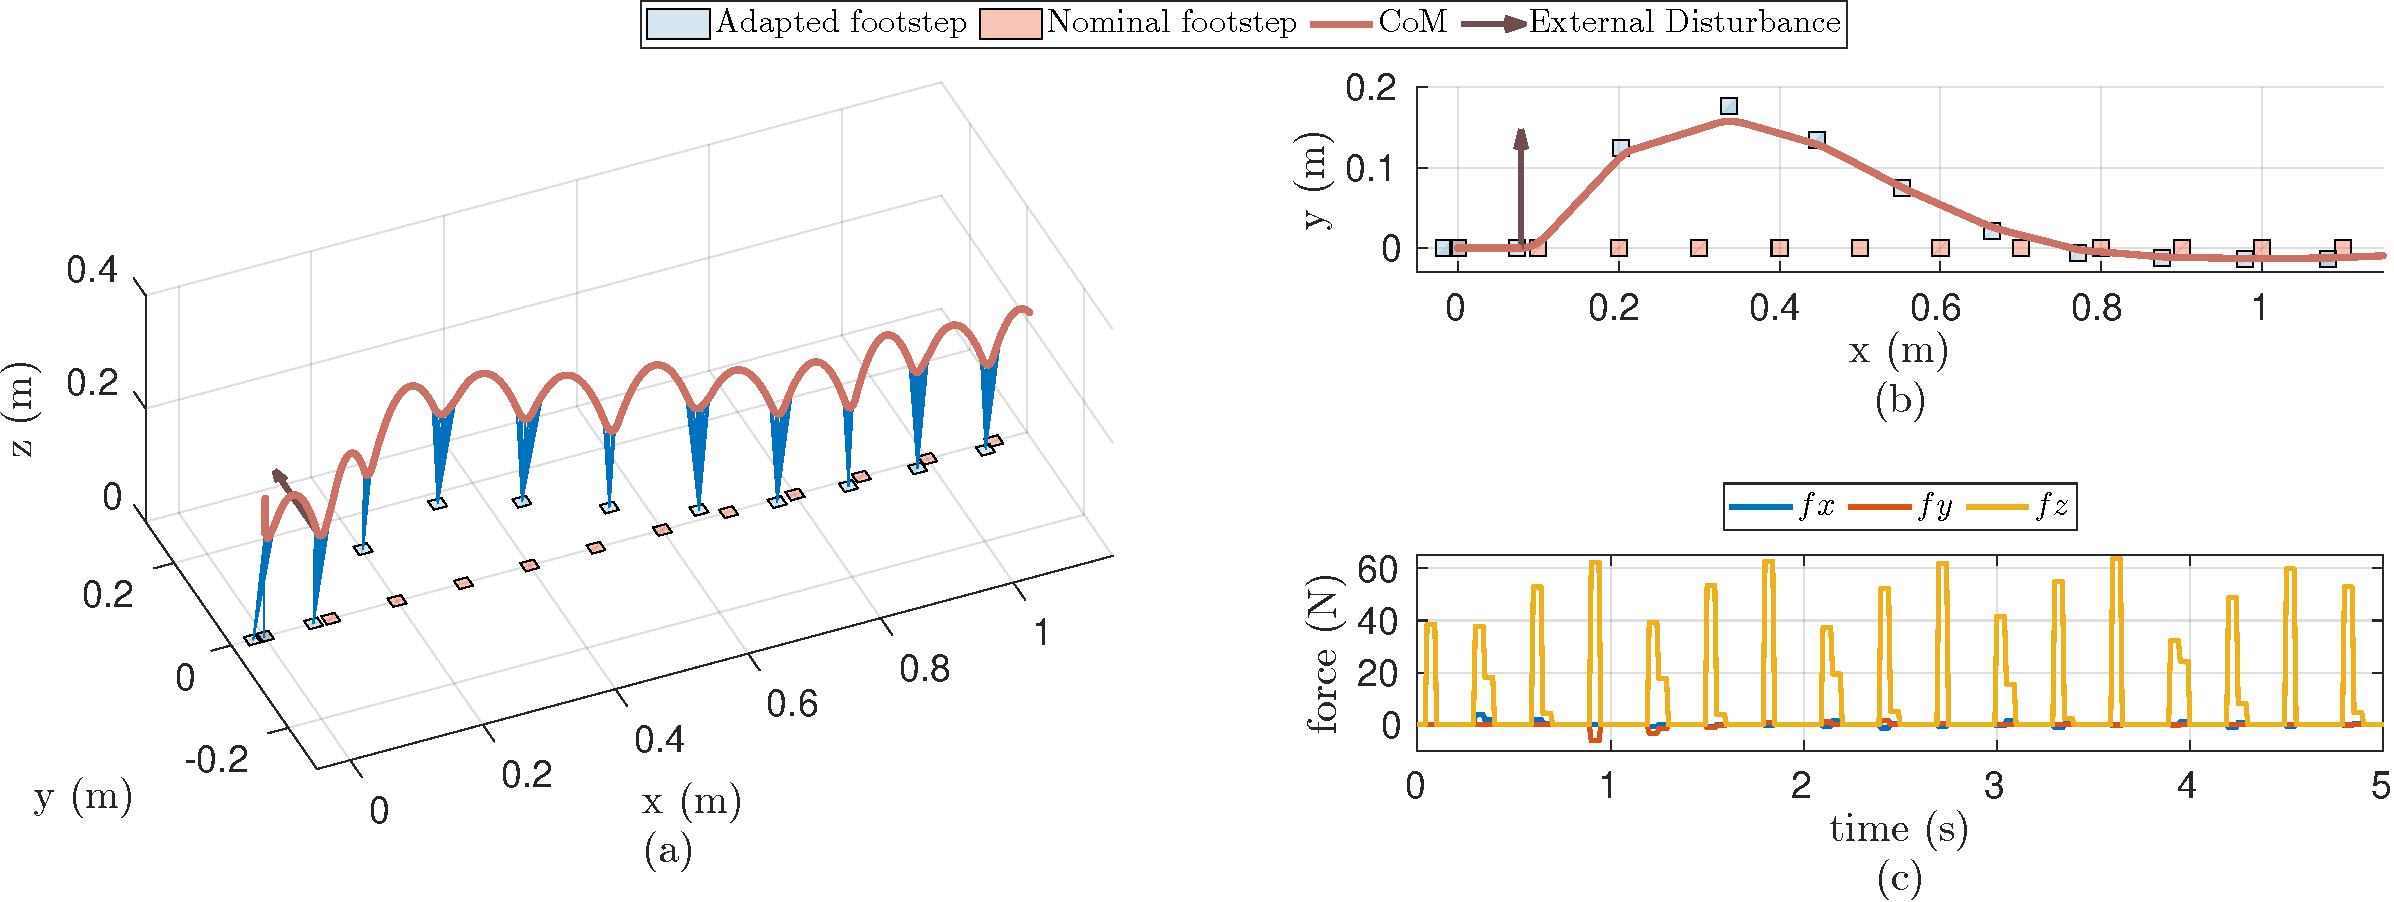
\includegraphics[width=\textwidth]{chapter_centroidal_mpc/figures/jump_traj.pdf}
    \end{myframe}
    \caption{(a)-(b) Trajectories generated by the MPC on a one-leg robot performing a jumping task. (c) Desired contact forces.}
    \label{fig:one_leg_jumping}
\end{figure}
\subsection{Reduced models simulation}
Figure~\ref{fig:one_leg_jumping} shows the trajectory generated by the centroidal MPC in the case of a floating base system equipped with one leg. The system has a mass of $\SI{1}{\kilo \gram}$ and the foot is approximated by a point, i.e., $n_c = 1$ and $n_v=1$ in Equation~\eqref{eq:centroidal_dynamics}. 
The MPC takes (on average) less than \SI{20}{\milli \second} for evaluating its output. At $t \approx \SI{1}{\second}$ an external force of magnitude $\SI{5}{\newton}$ acts for $\SI{0.5}{\second}$ at the system CoM.
The MPC automatically compensates 
\begin{figure}[!t]
    \centering
    \begin{myframe}{Two-legs running robot}
    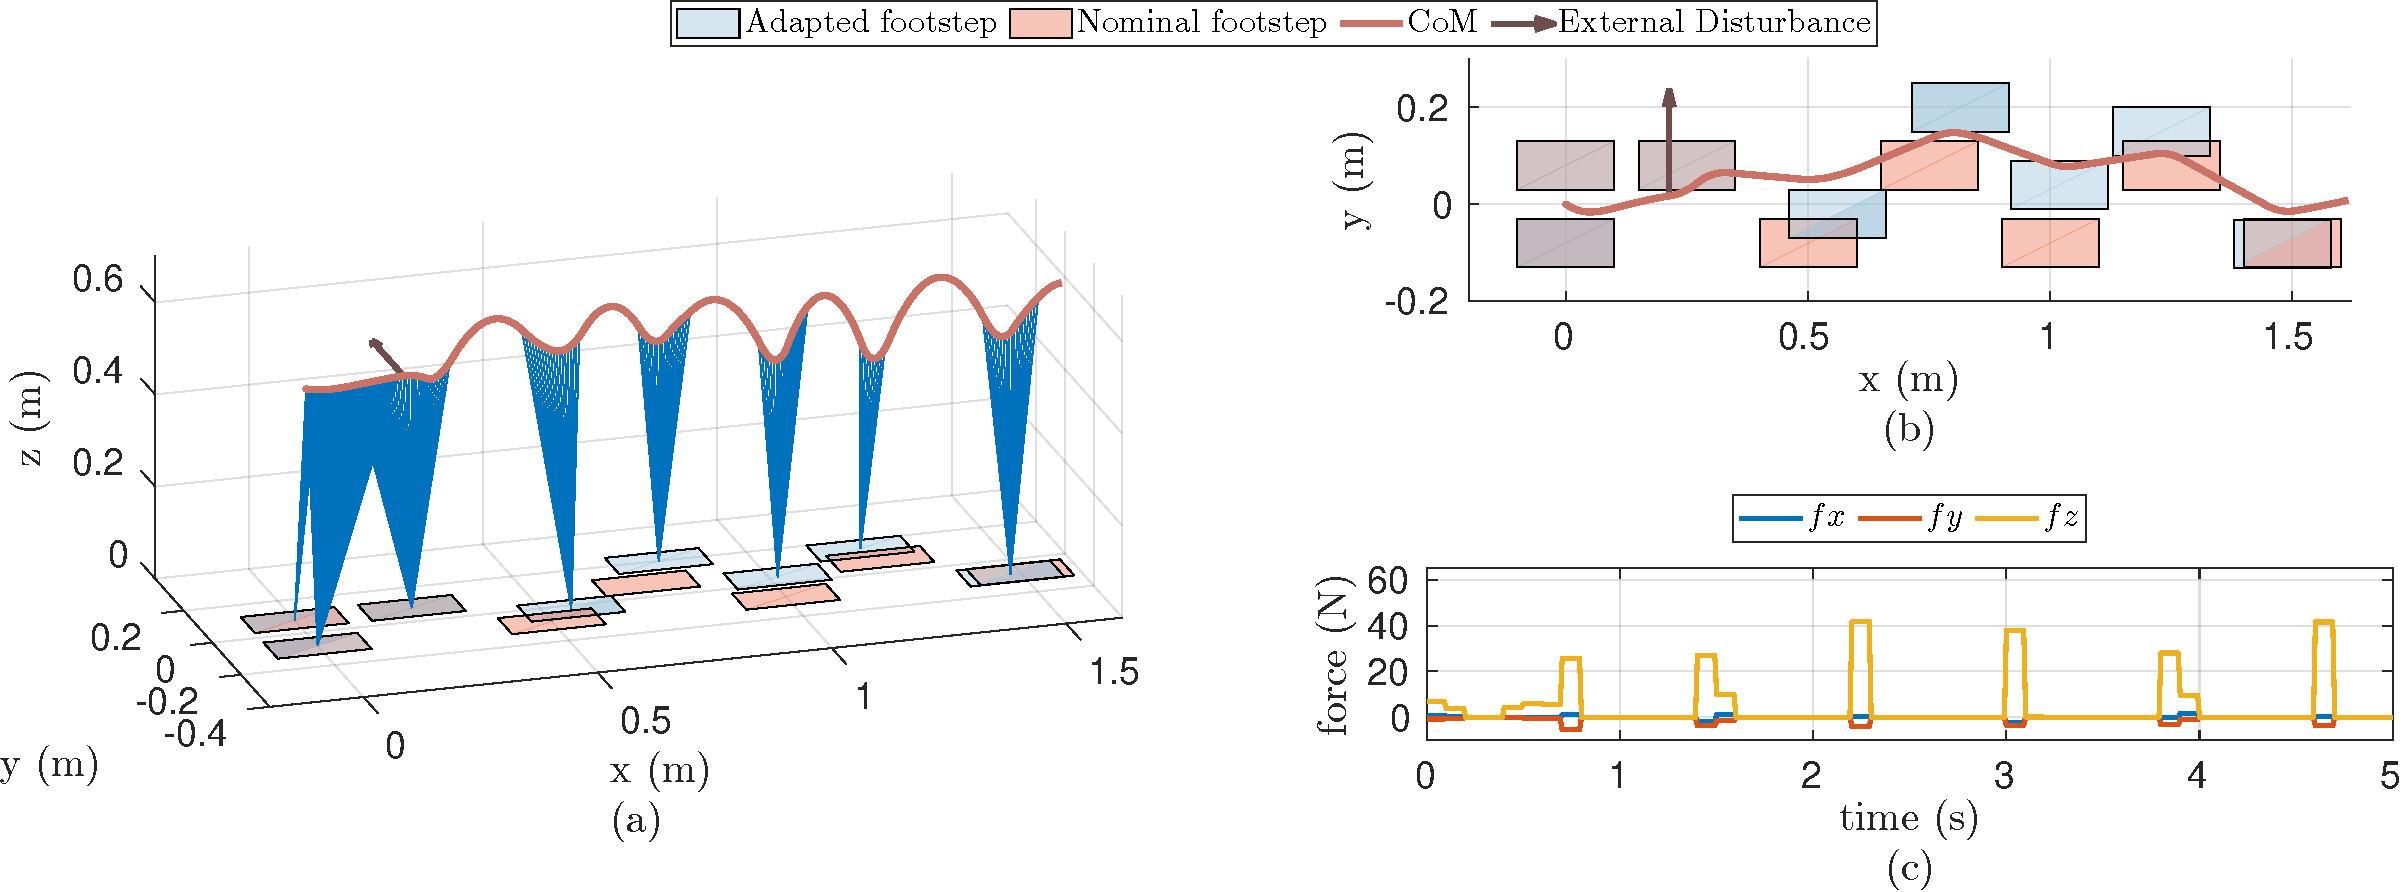
\includegraphics[width=\textwidth]{chapter_centroidal_mpc/figures/running_traj.pdf}
    \end{myframe}
    \caption{(a)-(b) Trajectories generated by the MPC on a two-legs robot performing a running task. (c) Desired contact forces.}
    \label{fig:running_traj}
\end{figure}
the disturbance effect by adapting the location of the footstep with an average of $\SI{10}{\centi \meter}$ - Figures~\ref{fig:one_leg_jumping}a and \ref{fig:one_leg_jumping}b.
Figure~\ref{fig:one_leg_jumping}c shows the contact force computed by the controller.
\par
Figure~\ref{fig:running_traj} presents the trajectory generated by the centroidal MPC in the case of a floating base system equipped with two legs. The system weighs $\SI{1}{\kilo \gram}$ and has a foot length and width of $\SI{20}{\centi \meter}$ and $\SI{10}{\centi \meter}$, respectively. In this case, $n_c = 2$ and $n_v=4$ in Equation~\eqref{eq:centroidal_dynamics}. The MPC takes (on average) less than \SI{80}{\milli \second} for evaluating its output. 
In this experiment, we analyze the capabilities of the MPC in the transition from locomotion to running. 
At $t \approx \SI{1}{\second}$ the planned contact sequence switches from a bipedal locomotion pattern, where a single support phase is always preceded by a double support phase, to a running pattern, where the single support phases are followed by aerial phases. Furthermore, at $t \approx \SI{1.5}{\second}$ an external force of magnitude $\SI{5}{\newton}$ acts for $\SI{0.5}{\second}$ at the robot CoM.
The MPC handles the transition from locomotion to running, while dealing with the external disturbance effect. Figs.~\ref{fig:running_traj}a and \ref{fig:running_traj}b show, in blue, the optimal contact location computed by the controller. The distance between the nominal contact and the computed one is (on average) $\SI{6}{\centi\meter}$.
Finally, Figure~\ref{fig:running_traj}c shows the contact force computed by the controller.


\subsection{Test on the iCub Humanoid Robot}
\begin{figure}[!t]
        \begin{subfigure}[b]{0.32\textwidth}
        \centering
        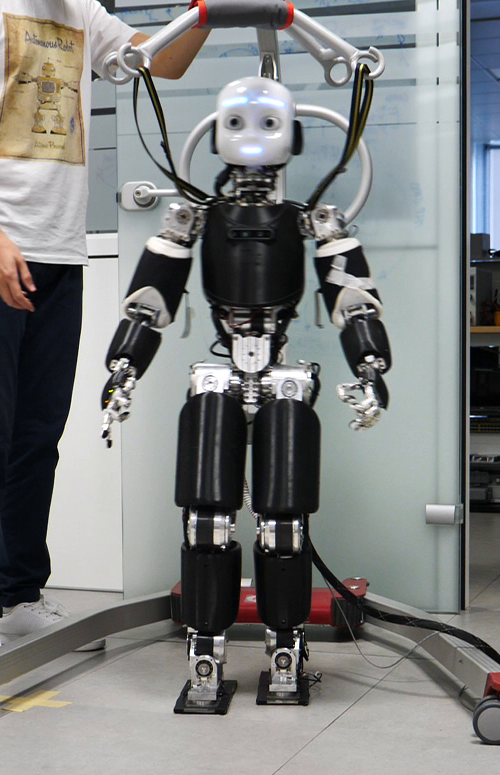
\includegraphics[width=\columnwidth]{chapter_centroidal_mpc/figures/icub1.png}
    \end{subfigure}
    \hfill
    \begin{subfigure}[b]{0.32\textwidth}
        \centering
        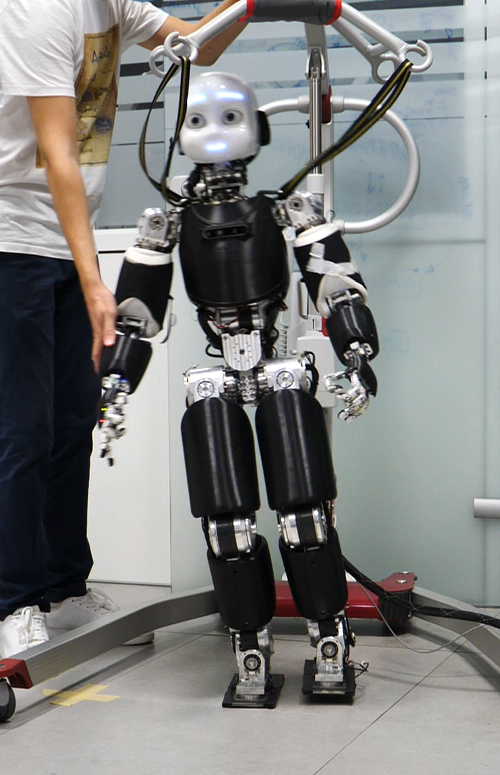
\includegraphics[width=\columnwidth]{chapter_centroidal_mpc/figures/icub2.png}
    \end{subfigure}
    \hfill
     \begin{subfigure}[b]{0.32\textwidth}
        \centering
        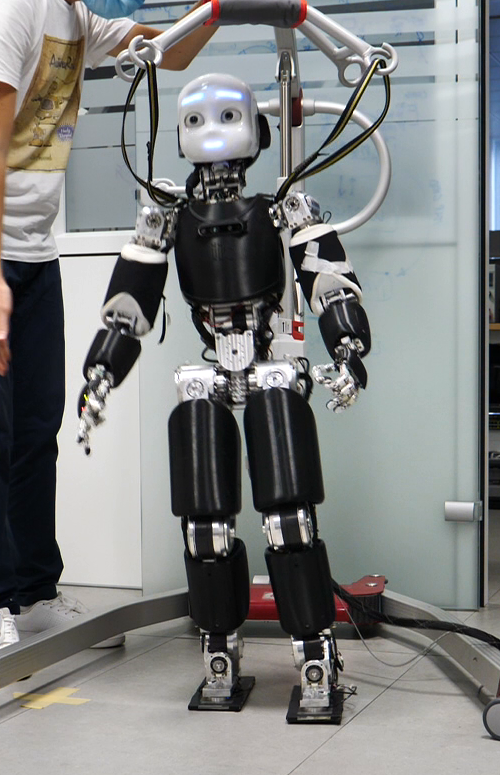
\includegraphics[width=\columnwidth]{chapter_centroidal_mpc/figures/icub3.png}
    \end{subfigure}
    \vskip 0.25cm
            \begin{subfigure}[b]{0.32\textwidth}
        \centering
        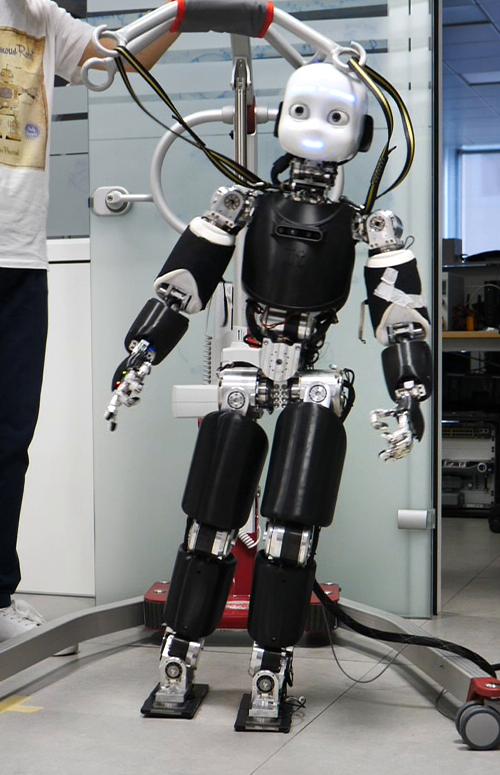
\includegraphics[width=\columnwidth]{chapter_centroidal_mpc/figures/icub4.png}
    \end{subfigure}
    \hfill
    \begin{subfigure}[b]{0.32\textwidth}
        \centering
        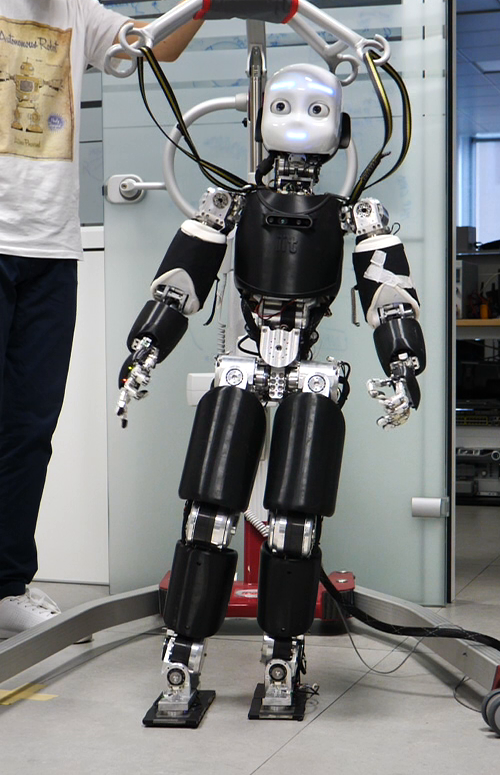
\includegraphics[width=\columnwidth]{chapter_centroidal_mpc/figures/icub5.png}
    \end{subfigure}
    \hfill
     \begin{subfigure}[b]{0.32\textwidth}
        \centering
        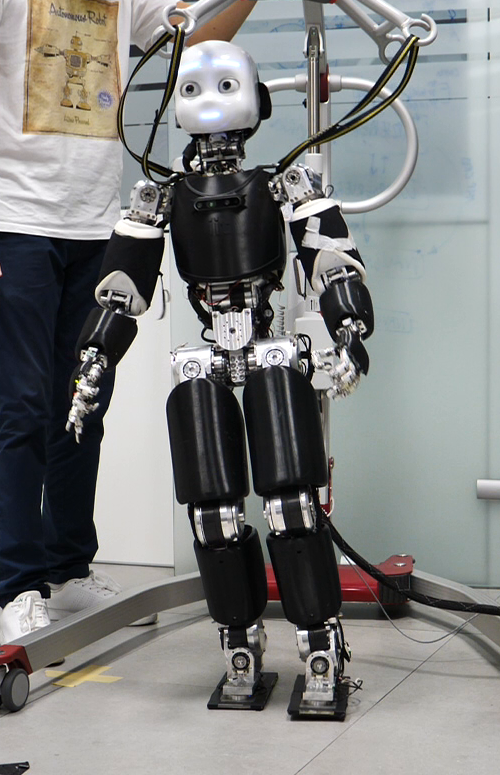
\includegraphics[width=\columnwidth]{chapter_centroidal_mpc/figures/icub6.png}
    \end{subfigure}
    \caption{The iCub humanoids robot react to an external disturbance.}
    \label{fig:icub3_centroidal_mpc}
\end{figure}

To validate the performance of the centroidal MPC on humanoid robots, we attached the controller to the three-layer architecture presented in Chapter~\ref{chapter:wbc_visco_elastic} and \ref{chapter:benchmarking_wbc} as show in Figure~\ref{fig:centroidal_mpc_architecture}.
In this scenario, \emph{trajectory optimization layer} is responsible for generating the nominal contact locations and timings. The nominal contact pose is considered as a regularization term for the contact position~\eqref{eq:task_contact} and to compute the regularized CoM trajectory~\eqref{eq:task_centroidal}.
The \emph{centroidal MPC} generates the feasible contact wrenches for the current active contacts and the new locations of the future active contacts. The future contact location is then set in the swing foot trajectory planner to generate a smooth trajectory for the foot. 
Finally, the inner \emph{whole-body control} loop evaluates the generalized velocity of the robot, $\nu$, by implementing the kinematics-based control law presented in Section~\ref{sec:ik_qp}. Here, the stack of tasks considers the references computed by the centroidal MPC.
As in Section~\ref{sec:ik_qp}, the tracking of the feet and the CoM trajectories are considered as high priority tasks, while the torso orientation is treated as a low priority task. Furthermore, to attempt the stabilization of the zero-dynamics of the system, a postural term is added as a low-priority task.
The joint velocities $\dot{s}$ included in the solution of the above problem are then integrated to obtain the joint position references for the low-level position controller. 
In our implementation, the whole-body control layer takes (on average) less than $\SI{1}{\milli \second}$ to evaluate its outputs.
\par
To analyze the step recovery capabilities of the whole architecture, the robot is perturbed by an external force acting on the right arm while walking. Since the robot is position controlled, it behaves rigidly when an external force is applied. Consequently, the position of the CoM is not perturbed. To mitigate this effect, we consider the estimated external force as a measured disturbance in the MPC. To do so, we modified the centroidal dynamics considered as the prediction model~\eqref{eq:centroidal_dynamics_discretized} as:
\begin{IEEEeqnarray}{cl}
\phantomsection     \label{eq:centroidal_dynamics_discretized_modified} \IEEEyesnumber \IEEEyessubnumber*
    {}_{\bar{G}} \dot{h} &=\sum_{i = 1}^{n_c} \sum_{j = 1}^{n_v} \begin{bmatrix}
      I_3 \\
      (p_{i} + R _{\mathcal{C} _ {i}}\; {}^{\mathcal{C}_i}  p_{v_{i,j}}  - x_{\text{CoM}})\times
    \end{bmatrix} \Gamma_i f_{i,j} + m\bar{g} + {}_{\bar{G}} \mathrm{f}_\text{ext} \\
    &=\mathcal{F}\left(p_{i}, x_{\text{CoM}}, f_{i,j}, {}_{\bar{G}} \mathrm{f}_\text{ext}\right).
\end{IEEEeqnarray}
where ${}_{\bar{G}} \mathrm{f}_\text{ext}$ is the measured external wrench expressed in the ${\bar{G}}$ frame. The measured contact wrench is considered different from zero only during the first index in the prediction horizon. in other words, in \eqref{eq:mpc_centroidal_centroidal_dynamics_optimization}, ${}_{\bar{G}} \mathrm{f}_\text{ext}[k] \ne 0$  only if $k = 0$.
\par
As shown in Figure~\ref{fig:icub_walking}c, the centroidal MPC takes less than $\SI{60}{\milli \second}$ to evaluate its output.
At $t \approx \SI{8}{\second}$ and $t\approx \SI{11}{\second}$ an external force of magnitude $\SI{40}{\newton}$ acts for $\SI{1}{\second}$ on the robot right arm -- second picture in Figure~\ref{fig:icub3_centroidal_mpc}.

The external force is estimated considering the Force Torque sensors mounted on the robot arms and the joint state applying the algorithm discussed in~\cite{Traversaro2017ModellingDynamics}. The MPC considers the external disturbance to propagate the centroidal dynamics~\eqref{eq:centroidal_dynamics_discretized_modified} and automatically compensates for the disturbance effect by adapting the location of the footstep with an average of $\SI{5}{\centi \meter}$ -- Figures~\ref{fig:icub_walking}a and \ref{fig:icub_walking}b.
\begin{figure}
    \centering
    \begin{myframe}{iCub walking}
    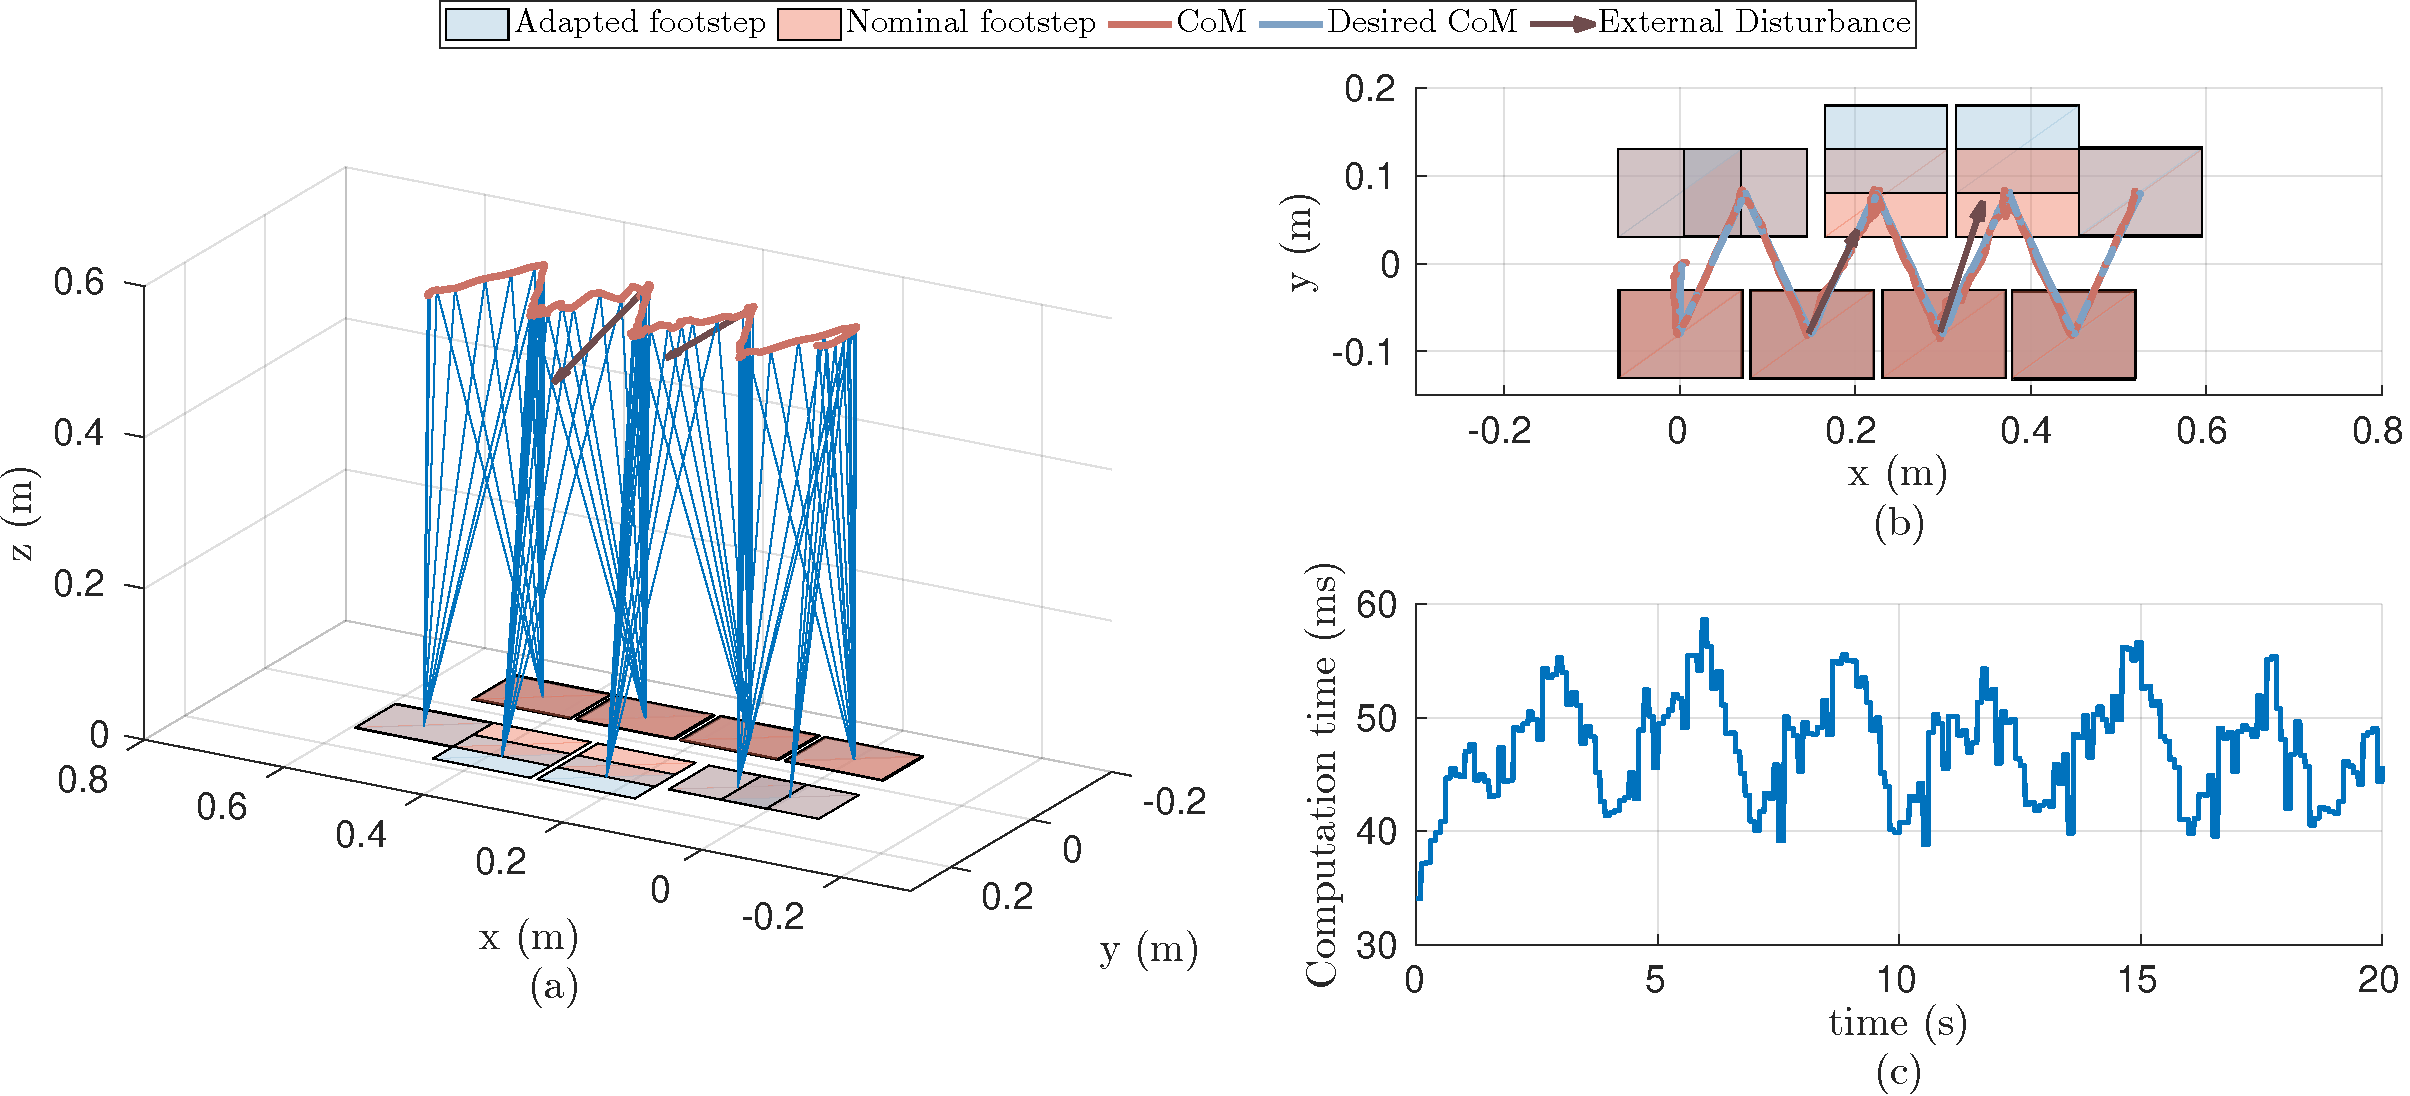
\includegraphics[width=0.945\textwidth]{chapter_centroidal_mpc/figures/icub_traj.pdf}
    \end{myframe}
    \caption{(a)-(b) Trajectories generated by the three-layer controller architecture on the iCub robot. (c) Computation time.}
    \label{fig:icub_walking}
\end{figure}